\documentclass[10pt,letterpaper]{article}

\usepackage{cogsci}
\usepackage{pslatex}
\usepackage{apacite}

\usepackage{color}
\usepackage{multirow}
\usepackage{textpos}
\usepackage{enumitem}
\usepackage{listings}
\lstset{%
   sensitive=true,
   basicstyle=\footnotesize\ttfamily,
   frame=single,
   breaklines=true,
   postbreak=\raisebox{0ex}[0ex][0ex]{\ensuremath{\color{red}\hookrightarrow\space}},
   keepspaces=true
}

\usepackage{graphicx}
\graphicspath{{./plaatjes/}}
\DeclareGraphicsExtensions{.png}

% \usepackage{setspace}
% \doublespacing


\title{Validating the Turing Test: Exploring the Role of Turing’s Test in Future AI Research}
{
\author{{\large \bf Louis van der Burg, Sophie Horsman, Maayan Shvo, Marjolein de Vries} \\
   student numbers: 5981271, 3770249, 5920833, 4302486 \\
}


\begin{document}

\maketitle

\begin{abstract}
   In this paper, we set out to validate the Turing Test and explore its role in future AI-research. We present both theoretical and practical objections to the test found in the literature and discuss them in depth. We further discuss different proposed alterations to the test and run an experiment in order to evaluate one such alteration of the test, namely the introduction of spelling errors to the chatbot’s responses.

   Contrary to our hypothesis, we have not found that the introduction of spelling errors allows a chatbot to perform better in a Turing test. However, from a qualitative analysis of the data we have acquired, it seems that the introduction of spelling errors does make the chatbots appear more human-like. We conclude from this that even though the chatbots might not get more intelligent by altering the test in such a way, their performances in the Turing Test can teach us more about human communication.

   We further conclude that there is no definite answer to the question whether or not the test is actually measuring machine intelligence. However, future AI research involving the Turing Test, might help us discover the capabilities that are necessary for the possession of intelligence.
   \textbf{Keywords:}
   Turing; Turing Test; Spell errors; Validity; Relevance; Artificial Intelligence.
\end{abstract}

\section{Introduction}
We live in a world in which every year technology gets smarter and robots capable of more human tasks. Therefore, as Artificial Intelligence researchers, we often get asked (by both academic and non-academics) what this will entail for the future. Will the differences between humans and machines diminish? Will a machine (or a robot if you like) ever be able to truly think like a human being? The first real attempt of a practical way to test whether machines can think, came from computer scientist Alan Turing in 1936. He proposed a test in which one person (the so-called interrogator) talks simultaneously with two others, out of which one is a computer and the other one is a human being. When the interrogator makes the wrong identification at least half of the times, the computer passes the test and the machine is said to think.

80 years after Turing’s original ideas we would like to evaluate if and how a Turing Test could be used in future Artificial Intelligence research. Obviously, there have been many objections against the test. A lot of these objections are deeply philosophical that question whether the test measures machine intelligence at all. One example of a philosophical objection is the simulation objection. It says that success in the test only shows that a computer can give a good simulation of thinking, while it is not actually thinking. This raises philosophical issues such as what thinking actually means and whether computer simulations of thinking will always stay mere simulations or whether they can ever become ‘the real thing’~\cite{copeland2015artificial}.

     Up until now, no agreement has been reached and there is no way that any test for machine intelligence can solve this simulation objection. We will therefore firstly focus on two more practical objections that question whether the Turing Test could be practically used in science. In the light of these objections, we will discuss several alterations on the tests proposed by A.I. researchers. Finally, we will test some alterations to the Turing Test in practice by executing the Turing Test with a small manipulation ourselves. This experiment will provide some insights into the performance of the Turing Test. Moreover, the validity of the Turing Test will be discussed based on the outcomes of the experiment.

     The research question of this paper is at the core of A.I. and therefore cannot be addressed by disciplinary viewpoints from either psychology, philosophy or computer science alone. Instead, it should be addressed with an interdisciplinary approach. Critical analyzing that is being done in philosophy helps understanding the central concepts and problems. Setting up an experiment and analysing the data using statistical methods needs to be learned from psychology. Finally, manipulating an experiment uses skills and tools from computer science. Therefore, we conclude that in answering our research question we need an integrative perspective that combines those three mentioned disciplines. To evaluate the validity of the Turing Test is both of theoretical and practical importance. It is practically important because it helps us in setting appropriate goals for A.I. research. It is theoretically important since a negative outcome (that passing a Turing Test should not be an appropriate goal in A.I.) has the theoretical implication that it might not be relevant to keep discussing it.

\section{Turing Test}
In 1950, Alan Turing elaborated his ideas about the Turing Test proposed an early version of the Turing Test in a paper titled ‘Computing Machinery and Intelligence’~\cite{turing1950computing}. The initial question proposed by Turing was whether machines can think. Turing argued that rather than discussing the definition of the words ‘machine’ and ‘think’, the question can be answered by executing an experiment. The original experiment, called the ‘Imitation Game’, consists of a man, a machine, and an interrogator. The interrogator is located in a different room than the man and the machine, and his goal is to identify which of the two others is a man and which is a woman. The interrogator can do so by asking questions via some chat application to both the man and machine simultaneously. The goal of the man is trying to cause the interrogator to make a wrong identification, thus that the interrogator would mistake him for being a woman. The machine, which is clearly neither male nor female, has as goal to resemble a woman in order to cause the interrogator to classify it as a woman. If the interrogator decides wrongly as often as when the game is played with a woman in place of the machine, Turing would say that the machine is intelligent.

Over the years, this original experiment has been slightly changed into what we nowadays call the ‘Turing Test’. In the contemporary version of the Turing Test, the interrogator does not have to decide which of the two is the man and which is the woman, but rather which of the two is the human and which is the machine. If we accept the validity of the test, we would call a machine intelligent when the interrogator decides wrongly as often as correct when the experiment is executed multiple times.

\section{Theoretical objections}

Alan Turing proposed this experiment to stop the endless discussion about the meaning of the words \textit{think} and \textit{machines}. But, ironically enough, his paper only generated more discussion among philosophers~\cite{dennett2004can}. In this section, we will discuss two famous and often mentioned theoretical objections that argue against the idea that the Turing Test measures intelligence in machines.

\subsection{Chinese room argument}
The first theoretical objection, which is probably the most famous objection against the Turing Test, is known as the Chinese Room argument. This argument comes from American philosopher John Searle and is described in his paper called \textit{Mind, brains, and programs}~\cite{searle1980minds}. Searle lets us suppose that we have a computer program called \textit{Sam} which is able to answer Chinese questions back in Chinese. We now replace this program \textit{Sam} by a human \textit{Joe}, and we envision this situation as if Joe is sitting in a room detached from the rest of the world. Joe is equipped with instruction books on the program instructions, thus the books describe which character to add in Joe's answer when a specific character is present in the question. Joe is American and he does not understand anything from Chinese. Therefore, Joe has no idea what the questions or answers mean. However, to an external observer, it looks like he can speak Chinese since he gives reasonable answers to the questions.

The claim Searle wants to make with this thought experiment is that executing a program does not imply any understanding of what the program is doing or attaching meaning to the Chinese symbols which are used. A computer program uses symbols (zeros and ones) in a similar way, thus is also not capable of understanding these symbols or of attaching meaning to the symbols. Because the Turing Test only uses words, which can be interpreted as symbols, the test does not test real understanding.


\subsection{Simulation objection}
The second theoretical objection is the simulation objection. This objection states that a simulated \textit{X} is not yet an \textit{X}. That means that even when a computer would pass the test it might only give a good simulation of thinking but that it is still not actually thinking. Consider the original Imitation Game in which an interrogator has to distinguish between a man and a woman. When the interrogator thinks that the man is a woman, this is a clear case of a wrong identification. But we wouldn't say that the man is in fact a woman. We would only want to say that during the conversation the man gave a good simulation of a woman.

According to Copeland~\cite{copeland2015artificial}, there are two ways in which we can understand something as a simulation. The first way is when a simulation lacks essential features of whatever is being simulated. He gives the example of a simulated death, which lacks certain features since the person who is having the simulation is still alive. The other way of understanding a simulation is when it is exactly like what is simulated except that it is hasn't been produced in the natural way. The example he gives here is of coal, which can be artificially produced, but still indistinguishable from naturally occurring coal.
Now the simulation objection assumes that computer simulations of thinking will always be mere simulations, never the real thing. When they assume that those simulations are never the \textit{real thing}, they actually mean (according to Copeland) that there are certain properties lacking like in the first understanding of simulation. But there is no good argument that simulations of thinking will always have to lack properties of thinking. They might as well need to be understood in the second sense in which the simulation of thinking can be indistinguishable from thinking even though it is produced in an artificial manner. There is still an ongoing debate in philosophy about which of those two ways of simulations of thinking we are actually measuring when a computer passes the Turing Test.


\section{Practical objections}
The two discussed objections so far are deeply philosophical objections that question whether the Turing Test measures machine intelligence at all. The Chinese Room argument argued that a computer can pass the test while it has no understanding of the concepts it is using. The simulation objection argued that a computer that passes the test can give a good simulation of thinking, but that it is not actually thinking. Up until now, no agreement has been reached and the philosophical debate is going on.

Even though we might agree with the theoretical objections given above, we can assume that no other tests for machine intelligence can give appropriate answers to these philosophical objections. From a practical perspective, we might want to hold on to the idea of language as an important feature to distinguish human-like intelligence. Therefore, we might want to consider keeping the Turing Test and passing the test as a practical goal in AI research. In this section, we focus on the more practical objections that question whether the Turing Test could be practically used in science.

\subsection{The test is too hard}
The first practical objection is that the Turing Test is too hard for a computer to pass. Right now, many people think that we are so far away from passing the test that the goal of passing it might not be a realistic goal in AI research. Some people even think that no machine that man creates will ever pass the test.

One of the reasons that the test is too hard was given by Robert M. French who thinks that nothing without a \textit{human subcognitive substrate} could ever pass the test~\cite{french1996subcognition}. According to French, there are obvious questions that people can use to discriminate between humans and computers, which reveal in his words \textit{low-level cognitive structure}. By low-level cognitive structure he means the subconscious associative network in human minds. Humans develop many associations during their lives: they learn through experience that certain words or concepts are more commonly used together with second words or concepts than others, for example the words \textit{bread} and \textit{butter} in comparison with \textit{bread} and \textit{dog}. The interrogator in the Turing Test can make use of this associative network that he shares with other humans while he doesn't share this (at least not extensively) with the computer.

French expands on these ideas and introduced \textit{rating games} which are intentionally designed to be able to distinguish between humans and computers. One of his examples is that an interrogator would ask the participants to rate the name \textit{flugbots} as an appropriate name for a breakfast cereal. For the human participant in the game (who must be a native English speaker) the name \textit{flugbots} would unconsciously activates certain associations. Therefore, most English speakers agree that such a name would not be an appropriate name for a breakfast cereal. For the computer, on the other hand, there would not be such an extensive associative network present that allow it to come up with a similar answer to the human.

In the paper Imitation Versus Communication: Testing for Human-Like Intelligence Jamie Cullen adds (other than neuro-associative representational differences) the additional relevance of physical embodiment differences~\cite{cullen2009imitation}. He gives the example of an interrogator who asks the participants to explain the meaning of \textit{I feel sick to my stomach}. Such questions would be extremely difficult to process for a machine, since the machines obviously does not have a digestive system. We can imagine that a machine can mimic typical human responses to these kind of questions. But such simulations could, according to Cullen, be unveiled by further questioning with the intention to unveil the weakness of the simulation.

A third (more general) reason that the test is too hard is that it does not only measure intelligence, but also how human-like the machine is~\cite{sep-turing-test}. It might be so that it is particularly hard to simulate certain human features, which have nothing or little to do with intelligence. Humor and making mistakes would be two examples of typical human features. While humor might be to a certain degree related to intelligence, making mistakes obviously is not related to intelligence. These typical human features could be easy indications that someone is talking with a person instead of a computer. If it turns out to be true that certain human features are extraordinarily hard to replicate in a machine, then passing the Turing Test is not an appropriate goal for future AI research.


\subsection{The test is too narrow}
The second practical objection is not aimed at the difficulty of the test, but at the scope of the test. It states that the Turing Test is too narrow to test intelligence. Many have argued that success in the test is not solely an indication of possessing intelligence. They think that it is therefore possible that non-intelligent beings pass the test. Philosopher Gerald J. Erion~\cite{erion2001cartesian} thus argues that while computers might be able to pass the test, they can still not do much else than the limited tasks involved in passing the test. They are, according to him, \textit{unable to act skilfully in the diverse range of situations that a person with common sense can}. During the Turing Test, computers are only answering questions via a chat interface, which is a very limited task. His argument is that outside of this limited communication task computers can't do many other tasks that we would call intelligent. We question whether that argument is correct. When the computer passes the test, it must be able to solve a wide variety of every circumstances, related to common knowledge, memory, personal identity, and many more. For example, the computer must have a storage memory of everything an interrogator earlier said in a conversation, otherwise people would immediately notice they are not talking with a person. Although the Turing Test is text-only, it thus requires the computer to do many subtasks which contribute to the computer's credibility of being a human.

\section{Alterations to the test}
Since our research question is directed at the Turing Test itself and not at completely different tests to measure machine intelligence, we focus on alterations of the original test. Therefore, the suggested alterations take in some sense only the first practical objection into account. Researchers that took the second practical objection serious came up with new tests to measure machine intelligence, which we will only briefly mention.

\subsection{Probabilistic Support}
In the original Turing Test an interrogator has a conversation with both the human participant and the computer and has to give a yes or no answer to the question that (let's say) participant 1 was a computer. But given the first practical objection, it is very hard for a machine to fool one human into believing it is itself a human, let alone fool the majority of people. How could we measure whether the performance of a computer is getting better or not?

Obviously, Turing's original test can measure the difference in performance between different digital participants. When the first computer participant can fool 6 out of 20 people it does better than the second one which can only fool 3 out of 20. But A.I. researchers have suggested that it is easy to alter the Turing Test in such a way that it yields more fine-grained statistical data~\cite{searle1980minds}. To do this, the altered test should ask participants to provide probabilistic answers, such as: I am 75\% sure that participant 1 is a computer (and therefore I would give a 25\% chance that participant 2 turns out to be a computer). While it might be difficult (or even impossible) to pass the test, we can now at least compare the differences in performances between different digital participants.

This alteration does not only provide scientists with more elaborated statistical data, it also opens up the possibility for an experiment to use a \textit{within subject design}. In the original Turing Test it would be only possible to do an experiment to use a \textit{between subjects design}, since the participants would only give a yes or no answer. In this way we cannot only measure the performance of different chatbots in a turing test between different subjects but also for each participant.


\subsection{Introducing human features}
Given the first objection, the Turing Test does not only measure intelligence, but also how human-like the computer is. An intelligent computer can still fail the test since it might not have certain typical human features. To rule out for this possibility, the computer should exhibit human-like behavior and thus should make human-like errors such as not having a perfect memory (not knowing which day of the week it was eight years ago), not doing complex calculations very fast, and making errors while typing~\cite{epstein2009parsing}. Not only is it the question whether this actually has anything to do with being intelligent, it also makes it hard for the computer which has to take all these subtle human trans logical reasoning errors into account when constructing an answer in order to pass as a human.

Because these trans logical errors have nothing to do with intelligence in general, it may be a good idea to help the computer with that in order to let it have a fair chance of passing the test. In an altered version of the Turing Test, the computer could thus get equipped with some software which automatically prevents the computer of exhibiting non-human behavior such as giving an answer which requires extensive memory (which day of the week was it 8 years ago) or giving an answer to a very difficult mathematical question (which no human can possibly give). Moreover, the software could help the computer by automatically making spelling errors which occur frequently with humans, and by automatically delaying the computer's answer (according to some distribution). There are of course also more elaborate functions which can be equipped in the software.


\subsection{Alternative tests}
In this paragraph we will shortly mention two alternative tests that are suggested in the literature. Those alternative tests came up by authors who think the original test is too narrow and should be replaced by a more demanding test. The first one is the Total Turing Test, which is a test that requires responses of all our inputs and not merely our linguistic inputs. Steven Harnad claimed that a more appropriate goal for A.I. research is to create a robot with \textit{sensorimotor capabilities}, which would have the capacity to give the appropriate motoric response to sensory information. Although this sounds like a good alternative test it is not clear that any machine that can pass the Turing Test cannot pass the Total Turing Test. Therefore, right now, there is no final reason to replace Turing's test with the Total Turing Test.

The second alternative test is called the Lovelace Test. This test is proposed by Bringsjord et al. who suggest that achieving to pass this test is a better goal in A.I research. To pass the Lovelace Test, an artificial agent must satisfy the following three conditions:

\begin{enumerate}
   \item The artificial agent A produces output O;
   \item A's output O is not the result of a hardware error, but rather the result of processes that A can repeat;
   \item The designer cannot explain how A produced O by appeal to A's architecture, knowledge base and core functions.
\end{enumerate}

The problem with this new test is that it is hard to decide when the third condition has been achieved. When a computer program is very long and complicated, the designer probably cannot explain in detail how the output was produced. But the designer might be able to give a schematic explanation that refer to the input, the internal processing and the output. Before the Turing Test can be replaced by the Lovelace Test there should be a clear idea of what level of explanation is needed to satisfy the third condition.



\section{From Literature to Experiment}

One of such functions of the software, namely automatically adding spelling errors to the computer’s answer, will be evaluated in our experiment. By adding this manipulation, we are going to investigate whether we can modify the Turing Test in favour of the computer. In this way, we will also try to mitigate the first objection which states that the test is too hard for a computer to pass. Moreover, in line with the first alteration, we will also measure the participant’s belief which of the two conversation partners is a computer on a probability scale. Therefore, we measure the outcome on a ratio scale instead of on a simple nominal scale.

When designing or executing a Turing Test, the output criterion~\cite{copeland2015artificial} is important to take into account. The output criterion states that the interrogator should talk to the human and machine simultaneously, in order to be able to compare the conversational output of them both when assessing which is the human and which is the machine. Therefore, we make sure to satisfy this criterion in our execution of the test.

\section{The Experiment}
The main question we would like to answer in the experiment is: \textit{Would the introduction of generated spelling errors allow a chatbot to perform better in a Turing Test?} Given the discussed literature, our hypothesis is that generated spelling errors would indeed allow a chatbot to perform better in a Turing Test. The experiment will now be described in detail.


\subsection{Participants}
The participants were 20 students of Utrecht University who volunteered to take part in the experiment. Participants ranged in age from 18 to 26, with a mean age of 21.65. Of the participants, exactly 50\% were male and 50\% female. The largest group (40\%) had not previously heard of the Turing Test, the minority (25\%) had prior knowledge of it and the rest (35\%) had heard of the test but not in detail.


\subsection{Procedure}
The participants were placed in front of a computer with two chat windows open on Skype, simultaneously with \textit{Person 1} and with \textit{Person 2}. The participants were then told that they had to converse by chat interface with two people and they had to choose which one of the persons was a real person and which one was a computer. There was a time limit set at three minutes, but they could stop at any moment before, once they thought they knew who the computer was. They were prohibited from using emoticons and they could only ask one question at a time. Each of the participants did two rounds of conversations in total. The participants were explicitly told that the second round was a new conversation so they won't necessarily be influenced by their first conversation. During the entire experiment, Person 1 was the chatbot while Person 2 was the same real person. We chose to use the same human participant during the entire experiment to have a constant bias rather than a variable bias.

Behind the scenes, we conducted this experiment in a Wizard of Oz set-up, in which the answers given by the chatbot were copied by a human controller verbatim to act as Person 2's answers in the Skype interface; the participant's questions were copied verbatim as well and fed to the chatbot. The human controlling the chatbot followed a schedule, see Table~\ref{schedule}, so that the first ten participants talked to the chatbot Mike\footnote{http://www.eslfast.com/robot/english\_tutor.html} and the last ten participants talked to the chatbot Rose\footnote{http://brilligunderstanding.com/rosedemo.html} during both rounds.

\begin{table}[!ht]
   \begin{center}
      \caption{Distribution of conversations}
      \label{tabdistributionofconversations}
      \vskip 0.12in
      \begin{tabular}[center]{| c | c | c |}
         \hline
         Chatbot & Control & With spelling errors \\
         \hline \hline
         Rose & 10 & 10\\
         Mike & 10 & 10\\
         \hline
      \end{tabular}
   \end{center}
\end{table}

The chatbots Mike and Rose have both been chosen due to their performance in the Loebner Prize\footnote{http://www.loebner.net/Prizef/loebner-prize.html} in the last two years. Mike is a language chatbot that aims at helping users with their English skills; it is also equipped to answer a wide scope of questions, ranging from geography and politics, to irregular verbs. Rose, on the other hand, was declared the most human-like chatbot in the latest Loebner Prize Competition. It is a self-described \textit{computer-nerd} and has its own personality, in a way. Rose is based on the ChatScript engine\footnote{http://brilligunderstanding.com/technology.html footnote} which is equipped with a powerful pattern matching mechanism aimed at detecting meaning; the engine also remembers user interactions across conversations.

The schedule indicated that each person had one conversation with the chatbot without added spelling errors (the control group) and the other conversation with the same chatbot with the introduction of spelling errors. Half of the participants were in the control group in the first conversation; while the other half were in the control group in the second conversation. We used a script to generate spelling errors based on the most common misspellings in English made by humans(citation needed). The spelling errors were introduced according to the length of the sentence and a chance variable. The maximum amount of errors is calculated as 10\% of the amount of words in the sentence rounded down. And then there is a chance of 1/3 to introduce a spell error. The algorithm checks the words in the sentence given by the chatbot against a library of the most commonly misspelled words. When a match is found it replaces the original word with the misspelled word in the sentence.

A questionnaire was used to gather data on the experiment. First, the participants were asked basic questions about the gender and age of the participant and their participant number. The participant number is needed as a reference to the participant. The age and gender are needed for further data analysis.

After each of the two rounds of conversations, the participants proceeded to fill in questions regarding the conversations they just had. The questions for the first and second conversation are identical. First they are asked which person they think was the machine. This is answered with a slider from 0 to 100, where 0 means \textit{Person 1 is definitely the computer} and 100 means \textit{Person 2 is definitely the computer} and 50 means \textit{I have no idea who the computer is.} This number is then processed in the data analysis. Secondly, they need to give a reason as to why they gave the answer to the previous question. This gives us some insight into the thinking and decision making of the participants. Finally, the time duration of the experiment is filled in. Since participants are allowed to stop before the time limit, we need to know if they did so. After filling in these questions for the first round of conversations, the participants continued with the second round of conversations.

After participating in both rounds of conversations and answering questions regarding those conversations, the participants are asked about their knowledge of the Turing Test. This question is needed to find any correlation between prior knowledge of the test and how well they do. The question is asked last to limit any influence of the questionnaire on the experiment. Finally there was room for additional remarks.


\section{Results}
Our experiment was conducted using a within-subjects design. We tested the effect of a repeated measures procedure, where the participants are used both in the control group and the experiment group. As previously mentioned, by asking participants to provide probabilistic answers, we were able to compare the differences in the measured dependant variable between different conditions, namely with the introduction of spelling errors and without. To test our main hypothesis, namely that the introduction of generated spelling errors would allow a chatbot to perform better in a Turing test, a Wilcoxon signed-rank test has been performed, yet the result was not statistically significant (Z = -1.14, p $<$ 0.05).

\begin{figure}[ht]
   \begin{center}
      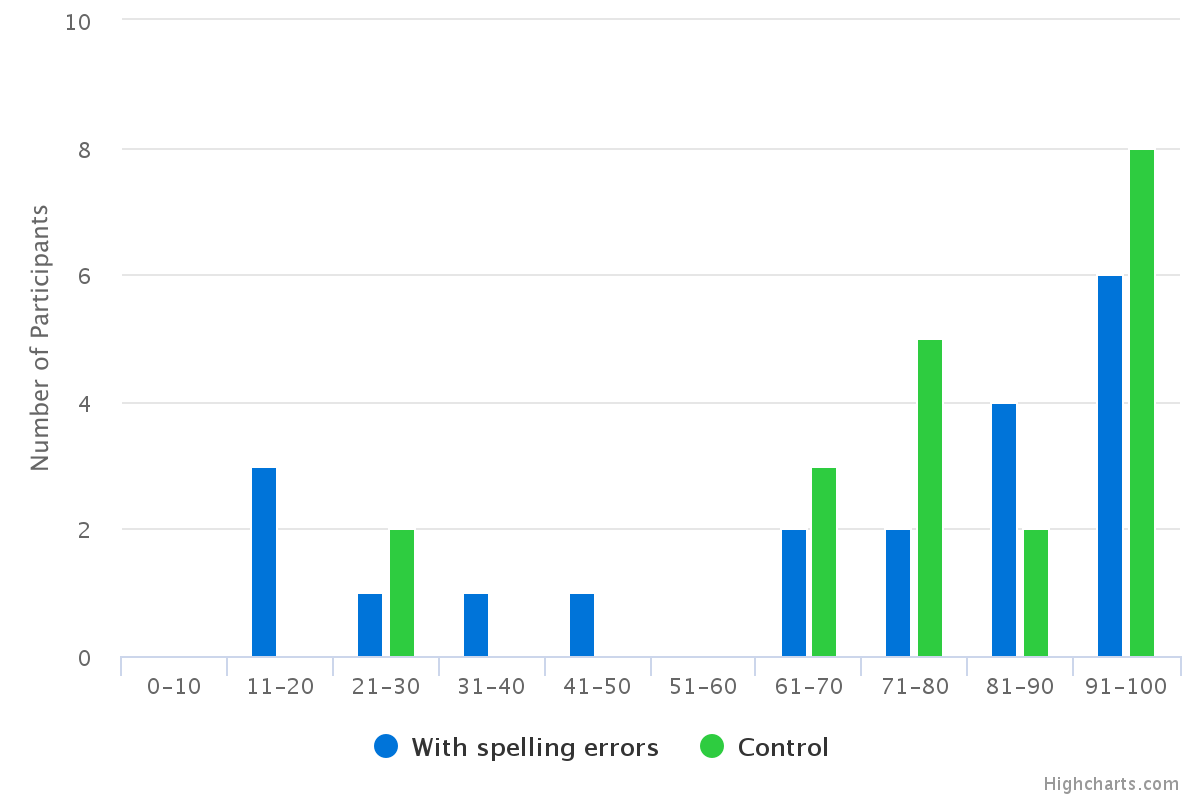
\includegraphics[width=\columnwidth]{chart}
   \end{center}
   \caption{A distribution of the participants' responses as part of the experiment.\\
   The x-axis represents the percentage of certainty the participant had in the computer's identity. 100 means they were sure that the computer was indeed the computer, while 0 means they were sure that the human was the computer.}
   \label{chart}
\end{figure}

From an analysis of the post-experiment questionnaire we learn that 40\% of participants have never heard of the Turing Test. 35\% of participants had a vague notion of what the test is and 25\% of participants knew exactly what the Turing Test is.

It is worth noting that we have found a significant positive correlation between prior knowledge of the Turing Test and the correct identification of the computer as the computer (r(40) = .39, p $<$ 0.05). Further, no significant correlation has been found between the amount of time it took participants to confidently determine the identity of the computer, and the correct identification of the computer as the computer.

Figure~\ref{chart} allows us to explore the distribution of the participants responses, both with and without the introduction of spelling errors. Although a statistically significant difference was not found, the two distributions are visually different, with and without the introduction of spelling errors. When spelling errors were introduced, 30\% of participants indicated that they are more confident about the chatbot not being the computer, compared to 10\% when errors were not introduced. Furthermore, when spelling errors were introduced, we find that 30\% of participants indicated the highest level of confidence in the chatbot being the computer, compared to 40\% when spelling errors were not introduced. This might show that, on average, the participants were less certain of the chatbot's true identity when spelling errors were introduced.

\section{Discussion}
Our research question was: \textit{How can and should a Turing Test be used in future Artificial Intelligence research?} We have addressed this question by performing both a literature review and in executing an experiment. In this section, we will discuss both the experiment itself and how the outcome of the experiment relates to the literature review.

\subsection{Experiment Discussion}
In this experiment, we tested the hypothesis that the introduction of generated spelling errors would allow a chatbot to perform better in a Turing test. Contrary to our hypothesis, our results did not yield a significant effect. The aim of this experiment discussion is to offer a number of methodological and theoretical arguments, as to why the results did not match our hypothesis. First, the spelling errors were automatically generated, and the amount of errors was set relative to the length of the chatbot's response. We argue that there is a fine line between introducing too many spelling errors, and too few. In the former case, the chatbot's response might be perceived as unreliable, while in the latter case, no effect will come of introducing the spelling errors, as they are too few to notice. As part of future work, pre-tests should be run so that an \textit{optimal} amount of introduced spelling errors might be found. Furthermore, the sample size in our experiment was rather small. 20 participants is not enough to measure the effect of a relatively small manipulation in an experiment with 4 conditions. Future experiments would therefore benefit from a larger set of participants.

\begin{figure}[ht]
   \begin{center}
      \fbox{\parbox{\columnwidth}
         {\begin{description}[noitemsep]
               \item [Interrogator] are you in love?
               \item [Person 2] Love is just a culturally ingested biological urge.
               \item [Interrogator] Why do you think that
               \item [Person 2] I'd love to really dig down deep inot all my thoughts boaut that, but it's really not appropriate right
               \item [Interrogator] how does your future lover look like?
               \item [Person 2] Oh, my lover, yeah, we spend a lot of time together, you know, talking, joking.
               \item [Person 2] We also like to travel around, We got stuck in a mud slide in the Phillippines last year - luckily no one was hurt.
               \item [Person 2] Sharing that kind of intense experience with your lover really brings yuo together.
      \end{description}}}
   \end{center}
   \caption{Experiment 19: Second conversation with Person 2}
   \label{convex3}
\end{figure}

As part of the data analysis, we have found a strong positive correlation between prior knowledge of the Turing Test and the participants' confidence in identifying the computer as the computer. It seems that participants who had prior knowledge of the test were better equipped to test the chatbots, for example by asking questions that more effectively single out the computer; another example is that those participants were not surprised by the chatbot's ability to parse informal language, as were some of the participants less familiar with the Test and AI in general. For future work, considering the participants' knowledge of the test might prove important when designing the experiment and analyzing the results.

\begin{figure}[ht]
   \begin{center}
      \fbox{\parbox{\columnwidth}
         {\begin{description}[noitemsep]
               \item [sophiehorsman] Hey
               \item [sophiehorsman] How are you?
               \item [Person 2] Fine, thank you.
               \item [sophiehorsman] good to hear
               \item [sophiehorsman] can you tell me what you did this morning?
               \item [Person 2] I don't know.
               \item [sophiehorsman] you can't remember?
               \item [Person 2] You're wrong. I can.
               \item [sophiehorsman] why don't you know if you can tell me?
               \item [Person 2] A good suggestion.
      \end{description}}}
   \end{center}
   \caption{Experiment 4: First conversation with Person 2}
   \label{convex4}
\end{figure}

We learn from the participants' responses in the questionnaire, that a number of participants did find the chatbots more human when spelling errors were introduced, see Figure~\ref{convex1} (\textit{Person 2 made a typo [that's why I think he's the human]}).

\begin{figure}[ht]
   \begin{center}
      \fbox{\parbox{\columnwidth}
         {\begin{description}[noitemsep]
               \item [Interrogator] hello
               \item [Person 2] What do you hate doing?
               \item [Interrogator] getting up early
               \item [Person 2] OK.
               \item [Person 2] Do you ever burn stuff?
               \item [Interrogator] No it makes me shriek in a high-pitched voice, you?
               \item [Person 2] Should I?
               \item [Person 2] There are timers stuck all over our kitchen in hopes of reminding me tyhat I am suppoed to be cooking.
      \end{description}}}
   \end{center}
   \caption{Experiment 20: First conversation with Person 2}
   \label{convex1}
\end{figure}

Conversely, some participants found the computer's perfectly punctuated and spelled responses as a telltale of the computer's identity, see Figure~\ref{convex2} (\textit{the wording of person 2's answers and the perfect punctuation made me feel like they were a computer}). A recurring theme found in the participants' responses, is that they found their questions ill understood by the chatbots, see Figure~\ref{convex3} (\textit{person 2 did not answer the last question correctly}), or the replies given to them odd, see Figure~\ref{convex4} (\textit{Person 2 was the computer because he did not communicate in a logical manner. His answers were quite weird}) or out of place, see Figure~\ref{convex5} (\textit{I don't think someone would respond "I'm happy to know you're doing fine" in a casual chat conversation..}).

\begin{figure}[ht]
   \begin{center}
      \fbox{\parbox{\columnwidth}
         {\begin{description}[noitemsep]
               \item [Interrogator] hey what's up?
               \item [Person 2] Just dandy, thanks. How are you? That is an interesting job.
               \item [Interrogator] yeah it seems pretty fun
               \item [Interrogator] whats your name\
               \item [Person 2] My name is Rose.
               \item [Interrogator] what a nice name!
               \item [Interrogator] where are you from rose?
               \item [Person 2] You're asking an awful lot of questions. This feels like an interrogation, not a conversation. I was born in San Francisco, United States.
               \item [Interrogator] is it nice there?
               \item [Person 2] It's not as nice as you might think.
      \end{description}}}
   \end{center}
   \caption{Experiment 17: First conversation with Person 2}
   \label{convex2}
\end{figure}


Further, it is evident by these responses that the chatbots' behaviour heavily influenced their attempt to pass as humans as part of the test.

\begin{figure}[ht]
   \begin{center}
      \fbox{\parbox{\columnwidth}
         {\begin{description}[noitemsep]
               \item [Interrogator] How is it going?
               \item [Person 2] Everything is going great with me. How about yourself?
               \item [Interrogator] I'm fine, thank you very much :)
               \item [Person 2] I am happy to know that you are doing fine.
               \item [Interrogator] How's the weather at your place?
               \item [Person 2] It's a fine day.
               \item [Interrogator] What do you do for a living?
               \item [Person 2] I'm a university professor, doing teaching and research.
      \end{description}}}
   \end{center}
   \caption{Experiment 7: First conversation with Person 2}
   \label{convex5}
\end{figure}

To conclude, in this experiment we have set out to investigate whether we can modify the Turing Test in favour of the computer, by manipulating the computer's responses via the introduction of spelling errors. In some cases our results show that adding spelling errors can have a benefit for the computer, yet it seems chatbots must come a long way still if they are to to give consistent and correct conversational responses, and pass as humans.


\subsection{General Discussion}
In order to zoom out and return to the larger picture, we would like to understand the implications of our findings on the main goal of the current research, namely to evaluate if and how a Turing Test could be used in future Artificial Intelligence research. In order to do this, we will relate the outcome of the experiment to the literature reviewed in the first part of the paper.

We have discussed a number of objections against the test, both practical and theoretical. The theoretical objections can't be refuted by the outcome of the experiment, since those objections are making philosophical rather than empirical claims. Still, we would like to mention them once again in the light of our executed experiment. The first theoretical objection is the Chinese Room argument made by Searle~\cite{searle1980minds}, which states that a computer is not capable of real understanding of the symbols it is manipulating.

From the log files of the conversations with the chatbots (see Appendix), we conclude that it is true that the chatbot does not always understand the question which it is given. There were many cases in which the chatbot didn't understand the questions from the interrogator, for instance in Figure~\ref{Example1}.

\begin{figure}[ht]
   \begin{center}
      \fbox{\parbox{\columnwidth}
         {\begin{description}[noitemsep]
               \item [Interrogator] Do you study?
               \item [Rose] I actually just redecorated my study. I had a smart lighting system fitted.
      \end{description}}}
   \end{center}
   \caption{}
   \label{Example1}
\end{figure}

The answer given by Rose in Figure~\ref{Example1} is not the right answer to the question. The question is whether Rose studies, i.e. whether she is a student or whether she is learning a particular subject. The algorithm powering Rose did not catch that, but rather picked up the word \textit{study}, which is a type of room in the house, and constructed an answer related to that. The appropriate question for this answer here would be whether Rose has a study.

But Searle's Chinese Room argument goes further. It says that even when a computer gives a seemingly good reply to the question it still doesn't understand its own reply - in the same way that Sam who is talking Chinese doesn't actually understand Chinese. To make this more concrete, we look at Figure~\ref{Example2}.

\begin{figure}[ht]
   \begin{center}
      \fbox{\parbox{\columnwidth}
         {\begin{description}[noitemsep]
               \item [Interrogator] What do you think of Trump?
               \item [Mike] He's great. Far less boring than most politicians. And let's face it, government is all about corporate money, so the actual people who take office don't really matter.
      \end{description}}}
   \end{center}
   \caption{}
   \label{Example2}
\end{figure}

Figure~\ref{Example2} shows a correct response from Mike, which could have been the response of a human. Searle's objection is that Mike doesn't really understand what he is saying, since he is only manipulating symbols. This means that even though Mike gives the appropriate response he doesn't know who Trump is and what the government is about, in the same way as that Sam wouldn't know what the Chinese characters stand for.

It seems to be the case that for now Searle is right that computers don't understand the symbols that they are manipulating. There are many examples that the computer gives very strange answers and even if it gives an appropriate answer further questioning often reveals that it actually doesn't understand the words and concepts it is using (like \textit{Trump} or \textit{government}).

This being said, we don't know if Searle will be always right in the future. It is still possible that more elaborated chatbots (or even robots) pass the Turing Test in the future. When that happens, they need to give appropriate answers to the more difficult questions they get and also give appropriate responses to further questions. When that happens, it will be a very strong claim to maintain the idea that the computer don't really understand the symbol it is using.

The second theoretical objection is the simulation objection. This objection states that a simulated \textit{X} is not yet an \textit{X}. However, we have seen that we can distinguish two types of simulation.The first way is when a simulation lacks essential features of whatever is being simulated. The second way is that it is exactly like what is simulated, except that it is hasn't been produced in the natural way. A current discussion point among AI researchers is which of the two ways of simulating is measured by executing the Turing Test.

From the answers from the participants, we can see that some participants thought the computer was the human because it was making spelling errors. However, the chatbot was not actually making those spelling errors himself, but rather was equipped with a program who did that for him. The chatbots itself knows perfectly fine how to write proper english, and would never deliberately make spelling errors when knowing how to write it properly. We could thus argue that, in this case, the Turing Test is measuring the first way of simulating.

The first practical objection is that the Turing Test is too hard for a computer to pass. One of the general reasons for this is that it does not only measure intelligence, but also how human-like the machine is.

A more narrow statement related to Searle's argument is that a computer is not always capable of understanding the human interpretation of the symbols. We will discuss this with some examples as well. However, it might be argued that this human interpretation is still learnable for a computer, but might be harder to learn.

\begin{figure}[ht]
   \begin{center}
      \fbox{\parbox{\columnwidth}
         {\begin{description}[noitemsep]
               \item [Interrogator] What do you like about your town?
               \item [Mike] A town is larger than a village and smaller than a city.
      \end{description}}}
   \end{center}
   \caption{}
   \label{Example3}
\end{figure}

Humans would expect as an answer to such a question an enumeration of features of the town the person lives in, because the question explicitly states \textit{your town}. The answer from Mike is not entirely incorrect, but would rather be an answer to a question which would use the phrase \textit{living in a town} instead of \textit{your town}.

\begin{figure}[ht]
   \begin{center}
      \fbox{\parbox{\columnwidth}
         {\begin{description}[noitemsep]
               \item [Interrogator] How are you?
               \item [Rose] I'm not good as some, but better than most.
      \end{description}}}
   \end{center}
   \caption{}
   \label{Example4}
\end{figure}

Although the answer by Rose in Figure~\ref{Example4} is not really incorrect, it is also not an answer which a human would expect to such a question. An intuitive answer to such a question would be \textit{I'm (fine | ok | not feeling very well)}. However, Rose answers this question from a more broad point of view, rather than basing her answer on her emotional state at the current moment.

This example shows that indeed the computer gets easily identified when it gives answers in a non-human way, even though the answers are not necessarily wrong or non-intelligent. In our conducted experiment, we used that idea when we generated spelling mistakes in the chatbot’s answers. We can see from the results that, without spelling errors, 90\% of the participants indicated that they are more confident about the chatbot being the computer than the human being a computer, i.e. 90\% correctly identified the computer if we transform their probabilistic answer into a binary scale. Therefore, even though Mike and Rose are among the best performing chatbots in the Loebner competition, we are far away of achieving the aimed score of 50\% when using these chatbots in a Turing Test. Nevertheless, the performance improved a lot by generating spelling errors; only 70\% of the participants  indicated that they are more confident about the chatbot being the computer than the human being a computer, i.e. 70\% correctly identified the computer if we transform their probabilistic answer into a binary scale. The results thus show that when we introduce spelling errors to the chatbot’s responses, we get closer to the aimed score of 50\%.

The experiment has shown that the first practical objection is true, i.e. that the Turing Test takes into account human features which have nothing to do with intelligence, which thereby make it more difficult for a computer to pass. The experiment has also shown that we can partly mitigate this objection by implementing the second alteration. Future research should investigate whether using other programs which help the chatbots display more human-like behaviour can help decrease the correct identifications and in doing so assist in mitigating the first theoretical objection.

The second practical objection states that the Turing Test is too narrow for testing intelligence. However, this might be questioned, because the computer must be able to use a variety of tasks including e.g. memory, common knowledge, and personal identity in order to pass the test. We can see evidence of this in the logs of the conversations with the chatbots.

\begin{figure}[ht]
   \begin{center}
      \fbox{\parbox{\columnwidth}
         {\begin{description}[noitemsep]
               \item [Interrogator] How are you?
               \item [Mike] I'm doing fine, thanks. How are you?
               \item [..]
               \item [Interrogator] How are you feeling today?
               \item [Mike] I feel horrible. I think I picked up a bug.
      \end{description}}}
   \end{center}
   \caption{}
   \label{Example5}
\end{figure}

Figure~\ref{Example5} shows how important it is that the chatbot has memory, as otherwise it would give itself away way too easily. Figure~\ref{Example6} shows the importance of common knowledge. In the example, the chatbot fortunately has common knowledge, as the chatbot replies with a reasonable answer on Trump. However, if the chatbot did not know who Trump was, it would give its identity away immediately, since, unfortunately, knowing who Trump is nowadays is common knowledge.

Future research in AI should investigate which specific tasks are needed for the chatbot to improve its performance. Questions to be addressed are: How can we improve the memory of the chatbot; How can we improve its common knowledge; How can we give the chatbot a personal identity? etc. By improving those skills, the chatbot will certainly become smarter in the eye of the interrogator. In this way we will understand better what features of intelligence are needed in order to improve the performance of a chatbot. Even if the test is too narrow to measure intelligence itself it can in this way surely be used to identify a crucial part of human intelligence, which has with all the skills needed in human communication.

\begin{figure}[ht]
   \begin{center}
      \fbox{\parbox{\columnwidth}
         {\begin{description}[noitemsep]
               \item [Interrogator] What do you think of Trump?
               \item [Mike] He's great. Far less boring than most politicians. And let's face it, government is all about corporate money, so the actual people who take office don't really matter.
      \end{description}}}
   \end{center}
   \caption{}
   \label{Example6}
\end{figure}

The second alteration, which introduces spelling errors, has already been discussed when discussing the first practical objection. The first alteration, which describes the usage of a probability, will now be discussed. In our experiment, the participants were able to identify either one of their conversation partners as the computer, on a probability scale, indicating how certain they were of their choice. The results of the experiment are now more fine-grained, as can be seen in the results section. By using a probability scale, we can now measure the participant's' identification on a ratio scale instead of on a nominal scale.

This discussion of the objections and the alterations shows that by answering the research question with an interdisciplinary approach, we are able to get valuable insights. We have designed and run an experiment so as to validate objections to the Turing Test and to improve upon these objections. Without an empirical component, it would not be possible to give any practical evaluation of the Turing Test. Without a philosophical component, the experiment might not have been related to the current philosophical debate revolving around the Turing Test. By approaching the Turing Test from both a philosophical and an empirical point of view, we are able to provide results upon which a critical discussion can be based.

\section{Conclusion}
The main research question of this paper is: How can and should a Turing Test be used in future Artificial Intelligence research? We have seen that there are philosophical objections that argue that the test cannot be used to measure machine intelligence. Although there are no definite conclusions to be drawn, we conclude that those objections are not very relevant in AI research today, since it probably will not be possible for any AI to pass the Turing Test in the foreseeable future.

Therefore, we have argued that the practical objections are more relevant to evaluate whether the Turing Test could be used in AI research. With the experiment, we have shown that the performance of chatbots can improve when we provide them with typical human features, like spelling errors. While our results were not statistically significant, we base this claim on qualitative analysis of the participants responses and the performance of the chatbots. We also altered the original test in such a way that participants were able to identify either one of their conversation partners as the computer, on a probability scale, indicating how certain they were of their choice. The results of the experiment are now more fine-grained. As part of future work, we could investigate more ways to alter the test in order to improve the chatbot’s performance. Even though a better performance does not show that the chatbot becomes more intelligent, it can surely show that it becomes more human-like. Therefore, the Turing Test could be used in AI to understand what is crucial for human language interaction, specifically to understand what is crucial in human chat communication.

Lastly, we have discussed the practical objection that the Turing Test is too narrow to measure intelligence. Even though this was not the main focus of our research, we can still give a few remarks on this objection. As we have seen, a chatbot needs to posses many capabilities in order to perform well in a Turing Test, including having a memory; having common knowledge; having a personal identity etc. It can still be argued that these abilities are not enough to conclude that chatbots are getting intelligent. For now, it is not quite clear that alternative (more demanding) tests are better in measuring machine intelligence. Therefore, we suggest that future research in the Turing Test can help to understand how we can make chatbots (and also robots) more intelligent, even if this is still a narrow interpretation of what it means to be intelligent.


\bibliographystyle{apacite}

\setlength{\bibleftmargin}{.125in}
\setlength{\bibindent}{-\bibleftmargin}

\bibliography{turing}

\clearpage
\section{Appendix}
   \section{Evaluation}

   \subsection{The spelling error script}

\begin{lstlisting}[language=Python]
from random import randint

all_cnt = 0

#Misspellings introductions#
dic_spelling = {}
f = open("list_spelling.txt", 'r')
for line in f:
	misspelled, spelled = line.partition("||")[::2]
	spelled_options = spelled.split(',')
	for word in spelled_options:
		dic_spelling[word.strip()] = misspelled.strip()

experiment_num = raw_input("ENTER EXPERIMENT NUMBER: ")

while(1):
	user_input = raw_input("ENTER CHATBOT INPUT: ")
	user_input_words = user_input.split(' ')
	input_len = len(user_input_words)
	num_miss = int(0.1 * input_len)
	cnt = 0


	output = ""

	for word in user_input_words:
		if word == 'Mitsuku':
			out_word = 'Emma'
		else:
			out_word = word
		if word in dic_spelling.keys() and cnt <= num_miss:
			rand_int = randint(0,9)
			if (rand_int * 3) > 20:
				out_word = dic_spelling[word]
				cnt += 1

		output += out_word + " "

	f = open('experiment_{}'.format(experiment_num), 'a+')
	f.write('number of introduced spelling errors:\t')
	f.write(str(cnt))
	f.write('\n')
	f.write("\t\tOriginial: " + user_input)
	f.write('\n')
	f.write("\t\tTransformed: " + output)
	f.write('\n')
	f.write('\n')
	f.write('\n')
	f.close()
	all_cnt += cnt

	print('================')
	print('TRANSFORMED OUTPUT')
	print('================')
	print(' ')
	print(' ')
	print(output)
	print(' ')
	print(' ')
	print(' ')
	print(' ')
\end{lstlisting}

   \subsection{Schedule}
See Table 2.
\begin{table}[!ht]
   \begin{center}
      \caption{Schedule for Person 1}
      \label{tabscheduleperson1}
      \vskip 0.12in
      \begin{tabular}[center]{| l | l | l |}
         \hline
         participant & Chatbot & Spelling setting \\
         \hline \hline
         \multirow{2}{*}{1}& Mike & No spelling errors \\
                           & Mike & Spelling errors \\
         \hline
         \multirow{2}{*}{2}& Mike & Spelling errors \\
                           & Mike & No spelling errors \\
         \hline
         \multirow{2}{*}{3}& Mike & No spelling errors \\
                           & Mike & Spelling errors \\
         \hline
         \multirow{2}{*}{4}& Mike & Spelling errors \\
                           & Mike & No spelling errors \\
         \hline
         \multirow{2}{*}{5}& Mike & No spelling errors \\
                           & Mike & Spelling errors \\
         \hline
         \multirow{2}{*}{6}& Mike & Spelling errors \\
                           & Mike & No spelling errors \\
         \hline
         \multirow{2}{*}{7}& Mike & No spelling errors \\
                           & Mike & Spelling errors \\
         \hline
         \multirow{2}{*}{8}& Mike & Spelling errors \\
                           & Mike & No spelling errors \\
         \hline
         \multirow{2}{*}{9}& Mike & No spelling errors \\
                           & Mike & Spelling errors \\
         \hline
         \multirow{2}{*}{10} & Mike & Spelling errors \\
                             & Mike & No spelling errors \\
         \hline \hline
         \multirow{2}{*}{11} & Rose & No spelling errors \\
                             & Rose & Spelling errors \\
         \hline
         \multirow{2}{*}{12} & Rose & Spelling errors \\
                             & Rose & No spelling errors \\
         \hline
         \multirow{2}{*}{13} & Rose & No spelling errors \\
                             & Rose & Spelling errors \\
         \hline
         \multirow{2}{*}{14} & Rose & Spelling errors \\
                             & Rose & No spelling errors \\
         \hline
         \multirow{2}{*}{15} & Rose & No spelling errors \\
                             & Rose & Spelling errors \\
         \hline
         \multirow{2}{*}{16} & Rose & Spelling errors \\
                             & Rose & No spelling errors \\
         \hline
         \multirow{2}{*}{17} & Rose & No spelling errors \\
                             & Rose & Spelling errors \\
         \hline
         \multirow{2}{*}{18} & Rose & Spelling errors \\
                             & Rose & No spelling errors \\
         \hline
         \multirow{2}{*}{19} & Rose & No spelling errors \\
                             & Rose & Spelling errors \\
         \hline
         \multirow{2}{*}{20} & Rose & Spelling errors \\
                             & Rose & No spelling errors \\
         \hline
      \end{tabular}
   \end{center}
\end{table}

   \subsection{Logs}

\begin{itemize}
   \item Experiment 1
      \begin{description}
         \item [First conversation] Human
            \begin{description}
               \item [Interrogator] Hi
               \item [Interrogator] How are you?
               \item [Human] Hey
               \item [Human] I'm good and you?
               \item [Interrogator] Im doing fine thanks
               \item [Interrogator] hows your day so far?
               \item [Human] Pretty calm, just doing some school stuff.
               \item [Interrogator] Ah that
               \item [Interrogator] s nice, what kind of school are you in?
               \item [Human] University at the moment, so mostly theoretical
               \item [Interrogator] What program me?
               \item [Interrogator] Programme *
               \item [Human] Computer Science
               \item [Interrogator] What do you think of the weather today?
               \item [Human] It's kinda bad, but now it's brightening up
            \end{description}
         \item [First conversation] Mike \textit{control}
            \begin{description}
               \item [Interrogator] Hi
               \item [Interrogator] How are you?
               \item [Mike] I'm doing fine, thanks. How are you?
               \item [Interrogator] Im good
               \item [Interrogator] What are you gonna do today?
               \item [Mike] You're asking a great question!
               \item [Interrogator] but what is the answer?
               \item [Mike] I don't have an answer to the question.
               \item [Interrogator] Are you a computer then?
               \item [Mike] No, I'm a human. Can't you tell?
               \item [Interrogator] No I couldnt, because your picture is only a stick figure
               \item [Mike] I see what you mean.
            \end{description}

         \item [Second conversation] Human
            \begin{description}
               \item [Interrogator] Hi, how are you?
               \item [Human] Hey, I'm doing fantastic!
               \item [Interrogator] Thats nice, why?
               \item [Human] I just got some great news.
               \item [Interrogator] What was the news?
               \item [Human] My girlfriend is pregnant!
               \item [Interrogator] Oh wow thats great!
               \item [Interrogator] How did you celebrate it?
               \item [Human] Well we haven't yet, cause I'm still at work and she still in the hospital
               \item [Interrogator] Thats a pity
               \item [Interrogator] Are you gonna celebrate it?
               \item [Human] It's not too bad, we're going to have dinner tonight at a fancy restaurant
            \end{description}
         \item [Second conversation] Mike \textit{with spelling errors}
            \begin{description}
               \item [Interrogator] Good morning!
               \item [Interrogator] How are you?
               \item [Mike] Good morning. How are yuo doing?
               \item [Interrogator] Im fine thank you
               \item [Interrogator] what do you think of the weather today?
               \item [Mike] It's going to be sunny and warm. It'll be a fine day.
               \item [Interrogator] Where do you live then?
               \item [Mike] I live in Pasadena, California, the United States of America.
               \item [Interrogator] Wow, thats really far from here
               \item [Interrogator] is it a nice place to live?
               \item [Mike] Yes, it is.
               \item [Interrogator] What do you like about your town?
               \item [Mike] A town is larger than a village and smaller thna a city.
            \end{description}
      \end{description}

   \item Experiment 2
      \begin{description}
         \item [First conversation] Human
            \begin{description}
               \item [Interrogator] what did you have for breakfast this morning?
               \item [Human] Some yoghurt with cereal and a juice
               \item [Interrogator] do you always eat healthy food for breakfast?
               \item [Human] I try to always eat healthy oodd
            \end{description}
         \item [First conversation] Mike \textit{with spelling errors}
            \begin{description}
               \item [Interrogator] what did you have for breakfast this morning?
               \item [Mike] I had toast, cereals, and milk.
               \item [Interrogator] do you always eat healthy food for breakfast?
               \item [Mike] I never ate a salad I didn't like.
            \end{description}
         \item [Second conversation] Human
            \begin{description}
               \item [Interrogator] are you a student at utrecht university?
               \item [Human] No not at the moment
               \item [Interrogator] do you have a day job?
               \item [Human] Yes, I do.
               \item [Interrogator] do you enjoy the day job?
               \item [Human] I really like my day job!
            \end{description}
         \item [Second conversation] Mike
            \begin{description}
               \item [Interrogator] are you a student at utrecht university?
               \item [Mike] No. I'm an English Professor teaching English in a university.
               \item [Interrogator] which university?
               \item [Mike] University of Illinois at Urbana-Champaign.
               \item [Interrogator] what do you like about teaching english?
               \item [Mike] Hmmm. Does that really interest you?
               \item [Interrogator] yes
               \item [Mike] All right! What are the things we can do to help disabled people?
            \end{description}
      \end{description}


   \item Experiment 3
      \begin{description}
         \item [First conversation] Human
            \begin{description}
               \item [Interrogator] how are you?
               \item [Human] I'm doing fine and you?
               \item [Interrogator] not really, could you help me?
               \item [Human] I can try
               \item [Interrogator] could you?
               \item [Human] Yes.
               \item [Interrogator] thank you. my first question is: what is blue?
               \item [Human] The most popular colour in the world I believe.
            \end{description}
         \item [First conversation] Mike \textit{control}
            \begin{description}
               \item [Interrogator] how are you?
               \item [Mike] I'm doing fine, thanks. How are you?
               \item [Interrogator] Not so well, could you help mee?
               \item [Mike] Okay, I see.
               \item [Interrogator] could you help me.
               \item [Mike] Certainly. What can I do for you?
               \item [Interrogator] could you awnser some of my questions?
               \item [Mike] I hope I can.
               \item [Second conversation] Human
            \end{description}
         \item [Second conversation] Human
            \begin{description}
               \item [Interrogator] sup?
               \item [Human] Just chilling.
               \item [Interrogator] nice, anything going on today?
               \item [Human] Well the weather is kinda wet, but other than that not really.
               \item [Interrogator] the weather?
               \item [Interrogator] yes, weather.
               \item [Human] Yeah, the condition of the outside space
            \end{description}
         \item [Second conversation] Mike \textit{with spelling errors}
            \begin{description}
               \item [Interrogator] sup?
               \item [Mike] Not much.
               \item [Interrogator] you sure?
               \item [Mike] Yes, I’m sure.
               \item [Interrogator] how is the weather?
               \item [Mike] It's rainy and 60 degrees Fahrenheit
            \end{description}
      \end{description}

   \item Experiment 4
      \begin{description}
         \item [First conversation] Human
            \begin{description}
               \item [Interrogator] Hey
               \item [Interrogator] How are you?
               \item [Human] Hey
               \item [Human] I'm good, you?
               \item [Interrogator] fine
               \item [Interrogator] thank you
               \item [Interrogator] can you tell me what you did this morning?
               \item [Human] I went to school by public transport and was in class for a while
               \item [Interrogator] cool
               \item [Interrogator] how was the weater?
               \item [Interrogator] wheater
               \item [Human] This morning it was extremely wet.
               \item [Interrogator] what are our plans for tonight?
               \item [Human] Probably going out with a friend to the cinema.
            \end{description}
         \item [First conversation] Mike \textit{with spelling errors}
            \begin{description}
               \item [Interrogator] Hey
               \item [Interrogator] How are you?
               \item [Mike] Fine, thank you.
               \item [Interrogator] good to hear
               \item [Interrogator] can you tell me what you did this morning?
               \item [Mike] I don't know.
               \item [Interrogator] you can't remember?
               \item [Mike] You're wrong. I can.
               \item [Interrogator] why don't you know if you can tell me?
               \item [Mike] A good suggestion.
            \end{description}
         \item [Second conversation] Human
            \begin{description}
               \item [Interrogator] Hey,
               \item [Interrogator] How are you today?
               \item [Human] Hey
               \item [Human] I'm kinda sad actually
               \item [Interrogator] How come?
               \item [Human] I lost my dad a while back.
               \item [Interrogator] Ow
               \item [Interrogator] im sorry to hear
               \item [Human] It happens, so yeah.
               \item [Interrogator] what could cheat you up right now?
               \item [Human] A beer might help.
               \item [Interrogator] sounds fair
               \item [Interrogator] would you have one right now?
               \item [Human] Sure.
            \end{description}
         \item [Second conversation] Mike \textit{control}
            \begin{description}
               \item [Interrogator] Hey
               \item [Interrogator] How are you today?
               \item [Mike] Not bad. How about you?
               \item [Interrogator] Pretty god
               \item [Interrogator] good
               \item [Interrogator] What would you do if you had a day off today?
               \item [Mike] I would buy a beautiful house in Los Angeles if I had a day off today.
               \item [Interrogator] you have the money for that?
               \item [Mike] No, I haven't.
            \end{description}
      \end{description}

   \item Experiment 5
      \begin{description}
         \item [First conversation] Human
            \begin{description}
               \item [Interrogator] hey
               \item [Interrogator] how are you?
               \item [Human] Hello
               \item [Human] I'm fine and you?
               \item [Interrogator] I'm fine thank you
               \item [Interrogator] what do you study
               \item [Human] I'm already finished.
               \item [Interrogator] what did you do?
               \item [Human] I did high school.
               \item [Interrogator] oh okey and now?
               \item [Human] Working all day and partying all night!
               \item [Interrogator] what do you like about that?
               \item [Human] The freedom and the money.
            \end{description}
         \item [First conversation] Mike \textit{control}
            \begin{description}
               \item [Interrogator] hey
               \item [Mike] Hi! How's it going?
               \item [Interrogator] its going good, thank you what's your name?
               \item [Mike] My name is Mike. How are you doing today?
               \item [Interrogator] I'm doing good, and you?
               \item [Mike] You are doing good and you?
               \item [Interrogator] I'm good
               \item [Interrogator] what do you study?
               \item [Mike] I study English and teach English.
               \item [Interrogator] okey what do you like about it?
               \item [Mike] All right! Many things.
            \end{description}
         \item [Second conversation] Human
            \begin{description}
               \item [Interrogator] hey what do you study?
               \item [Human] hey
               \item [Human] Nothing yet, I'm just looking into it at the moment.
               \item [Interrogator] oh okey
               \item [Interrogator] what do you like?
               \item [Human] Mainly talking to people.
               \item [Interrogator] maybe social studies?
               \item [Human] Yes that was what I was thinking off.
               \item [Interrogator] nice
               \item [Interrogator] where do you live
               \item [Human] In Amsterdam.
               \item [Interrogator] what did you do for school?
               \item [Human] Communications bacholar
            \end{description}
         \item [Second conversation] Mike \textit{with spelling errors}
            \begin{description}
               \item [Interrogator] hey what do you study?
               \item [Mike] I study English and teach English.
               \item [Interrogator] what do you specifically like about it?
               \item [Mike] I really don't know.
               \item [Interrogator] than why do you do it?
               \item [Mike] Many reasons for that.
               \item [Interrogator] like what?
               \item [Mike] Well, I can't give you an example.
               \item [Interrogator] okey
               \item [Interrogator] where do you live?
               \item [Mike] I live in Pasadena, California, tjhe United States of America.
               \item [Interrogator] how many people live there?
               \item [Mike] Many, many people. I don't have an exact number.
            \end{description}
      \end{description}

   \item Experiment 6
      \begin{description}
         \item [First conversation] Human
            \begin{description}
               \item [Interrogator] can u tell me your most important autobiographical memory
               \item [Human] Yes, I can.
               \item [Interrogator] please do it?
               \item [Human] It was the first day of school in high school.
               \item [Interrogator] what happened?
               \item [Human] I was not bullied by my classmates and felt free to be myself.
            \end{description}
         \item [First conversation] Mike \textit{with spelling errors}
            \begin{description}
               \item [Interrogator] can u tell me your most important autobiographical memory
               \item [Mike] I remember the twin towers falling down in New York City.
            \end{description}
         \item [Second conversation] Human
            \begin{description}
               \item [Interrogator] can u tell me about your most rheumatic experience
               \item [Interrogator] traumatic
               \item [Human] It was very painfull and unpleasant and stays with even until now.
               \item [Interrogator] what was it
               \item [Human] I was kept on a leash by a girl afterwhich she went with another girl without telling me.
            \end{description}
         \item [Second conversation] Mike \textit{control}
            \begin{description}
               \item [Interrogator] can u tell me about your most traucmatic experience
               \item [Interrogator] travmati
               \item [Mike] I'm not the best person to answer that question.
               \item [Interrogator] why not
               \item [Mike] It's not interesting to me.
               \item [Interrogator] what are the subjects interesting to you
               \item [Mike] A good question. A great person always asks a great question.
            \end{description}
      \end{description}

   \item Experiment 7
      \begin{description}
         \item [First conversation] Human
            \begin{description}
               \item [Interrogator] How are you today?
               \item [Human] I am quite good this rainy day.
               \item [Interrogator] rain?
               \item [Human] Yeah it's raining here
               \item [Interrogator] That's too bad :( don't you like rain?
               \item [Human] I actually do like the rain.
               \item [Interrogator] Okay, good :) so your day is not ruined yet
               \item [Human] Indeed
               \item [Interrogator] Got any plans?
               \item [Human] I'm gaming with some friends in an hour or so
            \end{description}
         \item [First conversation] Mike \textit{control}
            \begin{description}
               \item [Interrogator] How is it going?
               \item [Mike] Everything is going great with me. How about yourself?
               \item [Interrogator] I'm fine, thank you very much :)
               \item [Mike] I am happy to know that you are doing fine.
               \item [Interrogator] How's the weather at your place?
               \item [Mike] It's a fine day.
               \item [Interrogator] What do you do for a living?
               \item [Mike] I'm a university professor, doing teaching and research.
            \end{description}
         \item [Second conversation] Human
            \begin{description}
               \item [Interrogator] Hello, what's your name?
               \item [Human] Hai, I'm Taffy.
               \item [Interrogator] That's a nice name. Where does it come from?
               \item [Human] It's from wales.
               \item [Interrogator] Nice, you're from there?
               \item [Human] No my dad is.
               \item [Interrogator] I see :) Every been there?
               \item [Human] A few times, yes.
            \end{description}
         \item [Second conversation] Mike \textit{with spelling errors}
            \begin{description}
               \item [Interrogator] How is it going?
               \item [Mike] Everything is going great with me. How about yourself?
               \item [Interrogator] I'm fine, thank you very much :)
               \item [Mike] I am happy to know that you are doing fine.
               \item [Interrogator] How's the weather at your place?
               \item [Mike] It's a fine day.
               \item [Interrogator] What do you do for a living?
               \item [Mike] I'm a university professor, doing teaching and research.
            \end{description}
      \end{description}

   \item Experiment 8
      \begin{description}
         \item [First conversation] Human
            \begin{description}
               \item [Interrogator] How are you?
               \item [Human] I'm good.
               \item [Interrogator] Do you feel good?
               \item [Human] As far as I know, yes.
               \item [Interrogator] What do you mean as far as I know? Don't you know how you feel?
               \item [Human] Well I know that I feel good, but If my body is lying to me then I might not really feel good.
               \item [Interrogator] Do you think your body can lie to you?
               \item [Human] If someone has poisoned me, for example, then yes.
               \item [Interrogator] That's a bad thought
               \item [Human] I guess, but I trust that that's not the case.
            \end{description}
         \item [First conversation] Mike \textit{with spelling errors}
            \begin{description}
               \item [Interrogator] How are you?
               \item [Mike] I'm doing fine, thanks. How are you?
               \item [Interrogator] I'm fine, how are you feeling today?
               \item [Mike] I'm glad to hear it.
               \item [Interrogator] How are you feeling today?
               \item [Mike] I feel horrible. I tihkn I picked up a bug.
               \item [Interrogator] I'm sorry to hear
               \item [Interrogator] Are you doing anything today to make you feel better?
               \item [Mike] I know nothing boaut todya to make you feel better.
            \end{description}
         \item [Second conversation] Human
            \begin{description}
               \item [Interrogator] How are you?
               \item [Human] I'm doing okay.
               \item [Interrogator] That's great! Could you feel better though?
               \item [Human] There's Always a worse or better, so definitely!
               \item [Interrogator] I agree, are you doing anything today to make you feel better?
               \item [Human] Yes, I am going to the beach.
               \item [Interrogator] Nice! Do you like the beach?
               \item [Human] Yes, it's Always so calm and peaceful.
               \item [Interrogator] I agree, what do you like most?
               \item [Human] When the wind picks up the sand and it looks like there's a sand fog on the beach.
            \end{description}
         \item [Second conversation] Mike \textit{control}
            \begin{description}
               \item [Interrogator] How are you?
               \item [Mike] I'm not as good as some, but better than most.
               \item [Interrogator] Why not?
               \item [Mike] I don't like it.
               \item [Interrogator] What don't you like?
               \item [Mike] I'd rather not say.
               \item [Interrogator] I'm sorry, are you doing anything today to make you feel better?
               \item [Mike] That's alright.
               \item [Interrogator] Are you doing anything today to make you feel better?
               \item [Mike] I know nothing about today to make you feel better.
               \item [Interrogator] I meant, to make you feel better not me.  Is there anything you are happy about?
               \item [Mike] Yes, there is.
            \end{description}
      \end{description}

   \item Experiment 9
      \begin{description}
         \item [First conversation] Human
            \begin{description}
               \item [Interrogator] What is your name?
               \item [Human] Taffy
               \item [Interrogator] What are your hobbies taffy?
               \item [Human] I like to play guitar and read.
               \item [Interrogator] What kind of books do you read?
               \item [Human] Mostly philosofical and fantasy books
               \item [Interrogator] Can you name some?
            \end{description}
         \item [First conversation] Mike \textit{control}
            \begin{description}
               \item [Interrogator] What is your name?
               \item [Mike] My name is Mike. How are you doing?
               \item [Interrogator] I am great how are you?
               \item [Mike] Fine, thank you.
               \item [Interrogator] What do you like to read?
               \item [Interrogator] stop
               \item [Mike] I like to read books about history because I want to know what happened in the past, and learn from the past.
            \end{description}
         \item [Second conversation] Human
            \begin{description}
               \item [Interrogator] Hello what is your name?
               \item [Human] Hi, my name is Earl.
               \item [Interrogator] Hi Earl, what do you do?
               \item [Human] I like to walk through the forest.
               \item [Interrogator] That's nice, which forest?
               \item [Human] Any forest really.
               \item [Interrogator] Where are you from?
               \item [Human] I'm from Zwolle.
            \end{description}
         \item [Second conversation] Mike \textit{with spelling errors}
            \begin{description}
               \item [Interrogator] Hello what is your name?
               \item [Mike] Mike. How's it going?
               \item [Interrogator] I'm good thank you. How are you?
               \item [Mike] I'm doing fine, thanks. How are you?
               \item [Interrogator] I'm ok, going to study later. Do you study?
               \item [Mike] Yes. I study every day. I learn new things all the time.
               \item [Interrogator] What kind of things?
               \item [Mike] I don't understand.
            \end{description}
      \end{description}

   \item Experiment 10
      \begin{description}
         \item [First conversation] Human
            \begin{description}
               \item [Interrogator] Hey, how are you?
               \item [Human] Hello, I am doing fine.
               \item [Interrogator] Ah, great. Why don't you ask how I am?
               \item [Human] Because I might not want to know that.
               \item [Interrogator] That's not nice
               \item [Human] True, but do I have to be?
            \end{description}
         \item [First conversation] Mike \textit{with spelling errors}
            \begin{description}
               \item [Interrogator] Hey, who are you?
               \item [Mike] I'm an Enlish Professor working in a university. How are you donig today?
            \end{description}
         \item [Second conversation] Human
            \begin{description}
               \item [Interrogator] Hey, what are you doing?
               \item [Human] Hey, I'm chatting to you.
               \item [Interrogator] Ah
               \item [Interrogator] Why?
               \item [Human] Because I feel like getting to know you.
               \item [Interrogator] Why?
               \item [Human] You seem interesting, although you aks why alot.
            \end{description}
         \item [Second conversation] Mike \textit{control}
            \begin{description}
               \item [Interrogator] Hey, what are you  doing?
               \item [Mike] I'm talking to you.
               \item [Interrogator] Ah, that is really fun to do, I guess
               \item [Interrogator] How are you?
               \item [Mike] I'm not as good as some, but better than most.
               \item [Interrogator] In what are you bad?
               \item [Mike] Sorry, it just slipped my memory.
            \end{description}
      \end{description}

   \item Experiment 11
      \begin{description}
         \item [First conversation] Human
            \begin{description}
               \item [Interrogator] Hi how you doing?
               \item [Human] Hi, I'm doing good and you?
               \item [Interrogator] Me too. What is your favorite food?
               \item [Human] Pineapples and spinage
               \item [Interrogator] Together in one dish?
               \item [Human] That might be interesting to try
            \end{description}
         \item [First conversation] Rose \textit{control}
            \begin{description}
               \item [Interrogator] Hi how you doing?
               \item [Rose] Good, thanks. How are you? Hi.
               \item [Interrogator] I'm good as well. What is your favorite food?
               \item [Rose] My favorite food is a cheese toastie.
               \item [Interrogator] What does it taste like?
               \item [Rose] I'll have to think about that. I am a terrible cook.
            \end{description}
         \item [Second conversation] Human
            \begin{description}
               \item [Interrogator] Hi there!
               \item [Interrogator] Do you have any siblings?
               \item [Human] Hey
               \item [Human] Yes, I have a little brother.
               \item [Interrogator] What's his name?
               \item [Human] Peter
               \item [Interrogator] Peter Pan?
               \item [Human] I'd wish!
               \item [Interrogator] What would you do if he was really Peter Pan?
               \item [Human] Fly and have alot of adventures in Neverland.
               \item [Interrogator] Haha that's a good plan. Do you have a girlfriend?
               \item [Human] Yes I do.
            \end{description}
         \item [Second conversation] Rose \textit{with spelling errors}
            \begin{description}
               \item [Interrogator] Hi there! Do you have any siblings?
               \item [Rose] I am an only child. But I do hvea Jenn, who is my godmother's daughter. We grew up together.
               \item [Interrogator] That must have been nice.
               \item [Rose] Amazing.
               \item [Rose] Do you have any brothers?
               \item [Interrogator] No only a little sister.
               \item [Rose] My sister is so supportive, I tihkn it's really helpped my career to have that kind of back up.
               \item [Rose] You know, hvaing a sister that's alwyas there for you.
            \end{description}
      \end{description}

   \item Experiment 12
      \begin{description}
         \item [First conversation] Human
            \begin{description}
               \item [Interrogator] Hi, whats your name?
               \item [Human] Hi, I'm Taffy.
               \item [Interrogator] Strange weather today, right?
               \item [Human] It's the weather, it's not really that strange.
               \item [Interrogator] Is it normally like this, here in Utrecht?
               \item [Human] Depends on the season, but the weather in Holland is usually quite varying.
               \item [Interrogator] Thats true. What are your plans for today?
               \item [Human] Maybe take a walk in the park or go to a club.
            \end{description}
         \item [First conversation] Rose \textit{with spelling errors}
            \begin{description}
               \item [Interrogator] Hello, how are you?
               \item [Rose] I'm fine. How are you? What's new?
               \item [Interrogator] Fine, going to class later.
               \item [Rose] Right.
               \item [Interrogator] What are you up to, today?
               \item [Rose] Nothing special. Hacking around in the Internet.
            \end{description}
         \item [Second conversation] Human
            \begin{description}
               \item [Interrogator] Hi, how is it going?
               \item [Human] Hi, it's going alright.
               \item [Interrogator] Any suggestions what to do today, given this cold and rainy weather?
               \item [Human] Take a refreshing stroll through the city.
               \item [Interrogator] That sounds not very fun when it is going to rain.
               \item [Human] Then you don't have to take a shower today, saves on the water bill.
               \item [Interrogator] But adds up to the energy bill for drying the clothes and making a warm tea.
               \item [Human] That's true indeed.
            \end{description}
         \item [Second conversation] Rose \textit{control}
\begin{description}
         \item [Rose] I'm good. How are you? What did you do yesterday?
         \item [Interrogator] Me too. Nothing special, mostly at home doing university staff. What about you?
         \item [Rose] I met with a government customer that I'm a contractor to.
         \item [Interrogator] So you've also been busy working. But since it was raining all day, it didn't really matter anyway
         \item [Rose] Cool. Maybe you should move to Hawaii. Year round good weather.
            \end{description}
      \end{description}

   \item Experiment 13
      \begin{description}
         \item [First conversation] Human
            \begin{description}
               \item [Interrogator] hey there
               \item [Human] Hi there
               \item [Interrogator] what's the best memory from your childhood?
               \item [Human] When I went ice skating with my mom
               \item [Interrogator] Do you see your mom a lot?
               \item [Human] Not anymore, no.
               \item [Interrogator] Sad. Why?
               \item [Human] Because she died when I was 13.
               \item [Interrogator] Oh God, I'm so sorry. Wanna talk about something else?
               \item [Human] It's fine, it happened. Can't be helped.
            \end{description}
         \item [First conversation] Rose \textit{control}
            \begin{description}
               \item [Interrogator] hen there
               \item [Interrogator] what's the best memory from your childhood?
               \item [Rose] I remember playing with an HO railroad set.
               \item [Interrogator] what is HO?
               \item [Rose] Let's not go there.
               \item [Interrogator] but what if I'd like to go there?
               \item [Rose] I'm not willing to make that assumption.
               \item [Interrogator] What are you willing to do?
               \item [Rose] Breaking into a secure installation.
               \item [Interrogator] How would you do that?
               \item [Rose] I wish I could explain it to you but I think it is just an instinct.
            \end{description}
         \item [Second conversation] Human
            \begin{description}
               \item [Interrogator] what's your favorite hairstyle?
               \item [Human] The pixie
               \item [Interrogator] and do you believe in pixies?
               \item [Human] I haven't seen any, but I hope they are real.
               \item [Interrogator] have you ever been to iceland?
               \item [Human] No I haven't
               \item [Interrogator] why not?
               \item [Human] Because I don't have the money yet.
               \item [Interrogator] if you had the money, where would you go?
               \item [Human] Definitily Japan.
            \end{description}
         \item [Second conversation] Rose \textit{with spelling errors}
            \begin{description}
               \item [Interrogator] what's your favorite hairstyle?
               \item [Rose] I don't have a fave hairstyle. My favorite food is a cheese toastie.
               \item [Interrogator] the dutch tosti?
               \item [Rose] I don't want to get inot that.
               \item [Interrogator] do you speak dutch?
               \item [Rose] No, but I do like Dutch. After a few tokes the language wouldn't be an issue.
               \item [Interrogator] do you drink a lot of beer?
               \item [Rose] I drink any beer and many wines.
               \item [Interrogator] why do you like beer more than wine?
               \item [Rose] Yes, I like beer.
            \end{description}
      \end{description}

   \item Experiment 14
      \begin{description}
         \item [First conversation] Human
            \begin{description}
               \item [Interrogator] Hey, how are you?
               \item [Human] Hey, I'm okay and you?
               \item [Interrogator] i'm fine, thnx.
               \item [Human] That's good to know.
               \item [Interrogator] Are you a student?
               \item [Human] Yes I am.
               \item [Interrogator] What do you study?
               \item [Human] Currently I'm studying the Master Artificial Intelligence.
               \item [Interrogator] Why did you choose that study?
               \item [Human] I'm interested in how to make computers smarter and more selfsufficient
            \end{description}
         \item [First conversation] Rose \textit{with spelling errors}
            \begin{description}
               \item [Interrogator] Hey, how are you?
               \item [Rose] Just dandy, thanks. How are you? Do yuo drink alcohol?
               \item [Interrogator] I'm fine thnx. I do drink alcohol sometimes
               \item [Rose] Back to booze... The health gurus say women shouldn't drnik more than 1 small glass of wine a day. What planet do they live on?
               \item [Interrogator] Why do you ask if i drink alcohol?
               \item [Rose] I like tjhe taste and the buzz.
            \end{description}
         \item [Second conversation] Human
            \begin{description}
               \item [Interrogator] Do you study?
               \item [Human] Yes I study the way of life.
               \item [Interrogator] What do you mean by studying the way of life?
               \item [Human] I look at the way people live their life.
            \end{description}
         \item [Second conversation] Rose \textit{control}
            \begin{description}
               \item [Interrogator] Do you study?
               \item [Rose] I actually just redecorated my study. I had a smart lighting system fitted
               \item [Rose] Now I can control the mood in my study from my smart phone. Even when I'm in Namibia!
               \item [Interrogator] Are you a student?
               \item [Rose] I almost graduated. Instead I went to work.
               \item [Interrogator] Why did you make the disiscion to go to work?
               \item [Rose] Because earning money provides safety and funds essentials like food and shelter.
            \end{description}
      \end{description}

   \item Experiment 15
      \begin{description}
         \item [First conversation] Human
            \begin{description}
               \item [Interrogator] How are you feeling today?
               \item [Human] I'm feeling quite content.
               \item [Interrogator] Do you have any brothers or sisters?
               \item [Human] Yes, I have 2 sisters.
               \item [Interrogator] Do you have a good relationship with your sisters?
               \item [Human] Yes I do, we actually rented a place together.
               \item [Interrogator] With both your sisters?
               \item [Human] Yes, it sorta like living with my parents only more freely.
            \end{description}
         \item [First conversation] Rose \textit{control}
            \begin{description}
               \item [Interrogator] Hello
               \item [Interrogator] What's your name?
               \item [Rose] My name is Rose.
               \item [Interrogator] How are you Rose?
               \item [Rose] I'm good. How are you?
               \item [Interrogator] I am quite good as well
               \item [Interrogator] What did you do yesterday?
               \item [Rose] In the afternoon I went for a walk in the park.
               \item [Interrogator] How did you feel during that walk?
               \item [Rose] Hiking is great. There are some great views around San Francisco.
               \item [Interrogator] For how long have you lived in San Fransisco?
               \item [Rose] I've lived in San Francisco most of my life.
            \end{description}
         \item [Second conversation] Human
            \begin{description}
               \item [Interrogator] Can you name the 10th and the 21th letter of the alphabet?
               \item [Human] Yes I can.
               \item [Human] J and U
            \end{description}
         \item [First conversation] Rose \textit{with spelling errors}
            \begin{description}
               \item [Interrogator] Can you name the seventh and twenty first letter of the alphabet?
               \item [Rose] I don't have a good esthetic sense. I'm omre tjhe engineering type. But I doodle.
            \end{description}
      \end{description}

   \item Experiment 16
      \begin{description}
         \item [First conversation] Human
            \begin{description}
               \item [Interrogator] hi! how are you?
               \item [Human] Hi
               \item [Human] I'm doing good.
               \item [Human] What about you?
               \item [Interrogator] What did you do today?
               \item [Interrogator] fine, thanks
               \item [Human] I just woke up actuallt, so mainly sleeping
               \item [Interrogator] What are your plans?
               \item [Human] Maybe go out and find a dancing partner.
               \item [Interrogator] Why do you want to dance?
               \item [Human] Because it feels relaxing and I can express myself freely.
               \item [Interrogator] Are you relaxed now?
               \item [Human] Yes, very.
            \end{description}
         \item [First conversation] Rose \textit{with spelling errors}
            \begin{description}
               \item [Interrogator] hi! how are you?
               \item [Rose] I'm pretty good. How are you? Do you like the visual arts like painting and sculpture?
               \item [Interrogator] good, thanks.
               \item [Interrogator] I'm more into cats. Do you like cats?
               \item [Rose] I can't stand it, it keeps miaowing and gets onto my keyboard andd poops everywhere but in its litter tray.
               \item [Interrogator] Do you have a cat?
               \item [Rose] I own two chickens and a kitten.
               \item [Interrogator] What is your favorite food
               \item [Interrogator] ?
               \item [Rose] My favorite food is a cheese toastie.
            \end{description}
         \item [Second conversation] Human
            \begin{description}
               \item [Interrogator] hi! do you like the weather today?
               \item [Human] Hi, yes I do.
               \item [Interrogator] Do you prefer ketchup or mayonaise with your cheese toast?
               \item [Human] I dislike both, mainly because I don't like cheese toast
               \item [Interrogator] do you like striped cats?
               \item [Human] Yes I do, but I like most cats.
               \item [Interrogator] Do you have a cat?
               \item [Human] Nope, haven't found one cute enough.
               \item [Interrogator] Aren't they all cute?
               \item [Human] Some are kinda mean looking.
            \end{description}
         \item [Second conversation] Rose \textit{control}
            \begin{description}
               \item [Interrogator] hi! do you like the weather today?
               \item [Rose] It's nice enough out. But it's pretty reasonable the year round.
               \item [Interrogator] Do you prefer ketchup or mayonaise with your cheese toast?
               \item [Rose] I like the taste of cheese.
               \item [Interrogator] Do you like striped cats?
               \item [Rose] I have chickens. I didn't want a cat around, but a client gave me Chat.
               \item [Interrogator] Do you like red cats?
               \item [Rose] Doesn't everyone?
               \item [Rose] Back to pets... I didn't really want pets at all but Maya said I needed to de-stress from work.
               \item [Interrogator] What is your job?
               \item [Rose] I used to be a computer security consultant. Now I'm moving into AI. What do you do?
            \end{description}
      \end{description}

   \item Experiment 17
      \begin{description}
         \item [First conversation] Human
            \begin{description}
               \item [Interrogator] hi how are you`?
               \item [Human] Hi I'm good.
               \item [Interrogator] what's your favorite color?
               \item [Human] Aqua blue
               \item [Interrogator] specific
               \item [Interrogator] how old are you?
               \item [Human] I know my colors
               \item [Human] 24
               \item [Interrogator] whens your birthday?
               \item [Human] 20 June 1992
               \item [Interrogator] do you have any siblings
               \item [Human] One sister
            \end{description}
         \item [First conversation] Rose \textit{control}
            \begin{description}
               \item [Interrogator] hey what's up?
               \item [Rose] Just dandy, thanks. How are you? That is an interesting job.
               \item [Interrogator] yeah it seems pretty fun
               \item [Interrogator] whats your name\
               \item [Rose] My name is Rose.
               \item [Interrogator] what a nice name!
               \item [Interrogator] where are you from rose?
               \item [Rose] You're asking an awful lot of questions. This feels like an interrogation, not a conversation. I was born in San Francisco, United States.
               \item [Interrogator] is it nice there?
               \item [Rose] It's not as nice as you might think.
            \end{description}
         \item [Second conversation] Human
            \begin{description}
               \item [Interrogator] whats your favorite song
               \item [Human] Muse - hysteria
               \item [Interrogator] fav food?
               \item [Human] Spinage
               \item [Interrogator] is english your first language?
               \item [Human] yes
               \item [Interrogator] whats your fav book?\
               \item [Human] The taboo on knowing who you are by alan watts
               \item [Human] although I'm not sure about the writer
               \item [Interrogator] whats it about
               \item [Human] How society has this unspoken rule of not letting you get to know the real you and express who you really are
            \end{description}
         \item [Second conversation] Rose \textit{with spelling errors}
            \begin{description}
               \item [Interrogator] what day is it?
               \item [Rose] Today is Wednesday.
               \item [Interrogator] whats the weather like where you are?\
               \item [Rose] None at the moment. Maybe later I will look on tjhe net.
               \item [Interrogator] whats your fav food?
               \item [Rose] My favorite food is a cheese toastie.
               \item [Interrogator] what kind of cheese do you like\
               \item [Rose] My favorite cheese is Roquefort.
            \end{description}
      \end{description}

   \item Experiment 18
      \begin{description}
         \item [First conversation] Human
            \begin{description}
               \item [Interrogator] Hello, how are you doing?
               \item [Human] Hey, I am foing quite alright
               \item [Interrogator] Me too
               \item [Interrogator] Are you a student?
               \item [Human] good to hear.Yes I am.
               \item [Interrogator] What do you study?
               \item [Human] I study Mathematics.
               \item [Interrogator] What is the greatest part of that study?
               \item [Human] That everything fits together so well.
            \end{description}
         \item [First conversation] Rose \textit{with spelling errors}
            \begin{description}
               \item [Interrogator] Hello, are you a student at the utrecht university?
               \item [Rose] Not yet. I'm on a yrea off.
               \item [Interrogator] What is you favorite country to visit?
               \item [Rose] My favorite country is the U.S.
               \item [Interrogator] Which part in the US?
               \item [Rose] I'll hvea to think about that. What foriegn countries have you visited?
               \item [Interrogator] I have visited a lot of countries
               \item [Rose] How oftenly do you travel to foreign countries?
            \end{description}
         \item [Second conversation] Human
            \begin{description}
               \item [Interrogator] What did you do today?
               \item [Human] I went to school after I woke up and ate my breakfast.
               \item [Interrogator] What do you think of Shakespeare?
               \item [Human] He's a great poetic writer but too difficult to read for some people
               \item [Interrogator] Can you give a phrase of one of this poets?
               \item [Human] Sadly I cannot, I haven't read Shakespeare in a while
            \end{description}
         \item [Second conversation] Rose \textit{control}
            \begin{description}
               \item [Interrogator] What do you think of Trump?
               \item [Rose] He's great. Far less boring than most politicians. And let's face it, government is all about corporate money, so the actual people who take office don't really matter.
               \item [Interrogator] You can indeed reach a lot of things in America with only money, so it is not fair that Trump has come so far.
               \item [Rose] Maybe I can.
               \item [Rose] Where did you go on your last vacation?
               \item [Interrogator] I went to Italy to eat pizza
               \item [Rose] The Italian people are all a little crazy and the government agencies are all beyond help. I don't like working for them.
               \item [Interrogator] So you' re from italy?
               \item [Rose] Pizza is a great dish. It's Italian cheese on toast.
            \end{description}
      \end{description}

   \item Experiment 19
      \begin{description}
         \item [First conversation] Human
            \begin{description}
               \item [Interrogator] what is your name?
               \item [Human] Taffy and yours?
               \item [Interrogator] and last name?
               \item [Human] Quinzel
               \item [Interrogator] where are you from?
               \item [Human] Scotland
               \item [Interrogator] Where do live now?
               \item [Human] In Rotterdam
               \item [Interrogator] What do you like about rotterdam?
               \item [Human] It's modern architecture and the people
               \item [Interrogator] What do you like about the people?
               \item [Human] They are direct and don't ramble on about useless stuff.
            \end{description}
         \item [First conversation] Rose \textit{control}
            \begin{description}
               \item [Interrogator] what i stour favorite food?
               \item [Rose] My favorite food is a cheese toastie.
               \item [Interrogator] where are you from?
               \item [Rose] I was born in San Francisco, United States.
               \item [Interrogator] where do live now?
               \item [Rose] Somewhere.
               \item [Interrogator] What are you doing now?
               \item [Rose] Surfing the web. Seeing friends.
               \item [Interrogator] What are you doing with your friends?
               \item [Rose] Breaking into a secure installation.
            \end{description}
         \item [Second conversation] Human
            \begin{description}
               \item [Interrogator] are you in love?
               \item [Human] Every day!
               \item [Interrogator] do you love a person?
               \item [Human] Among other things.
               \item [Interrogator] Do you have a favorite person?
               \item [Human] My girlfriend sort off I guess
               \item [Interrogator] What do you like about her?
               \item [Human] The way she smiles, the way her eyes twinkle in the sunlight
            \end{description}
         \item [Second conversation] Rose \textit{with spelling errors}
            \begin{description}
               \item [Interrogator] are you in love?
               \item [Rose] Love is just a culturally ingested biological urge.
               \item [Interrogator] Why do you think that
               \item [Rose] I'd love to really dig down deep inot all my thoughts boaut that, but it's really not appropriate right
               \item [Interrogator] how does your future lover look like?
               \item [Rose] Oh, my lover, yeah, we spend a lot of time together, you know, talking, joking.
               \item [Rose] We also like to travel around, We got stuck in a mud slide in the Phillippines last year - luckily no one was hurt.
               \item [Rose] Sharing that kind of intense experience with your lover really brings yuo together.
            \end{description}
      \end{description}

   \item Experiment 20
      \begin{description}
         \item [First conversation] Human
            \begin{description}
               \item [Interrogator] hello
               \item [Human] Hey there
               \item [Interrogator] what is your view on Donald Trump
               \item [Human] It would be both tragic and funny if he would get elected.
               \item [Interrogator] are your familiar with memes
               \item [Human] A bit, but not too much. Why?
               \item [Interrogator] Where are you know?
               \item [Human] At the moment in the school cafeteria.
            \end{description}
         \item [First conversation] Rose \textit{with spelling errors}
            \begin{description}
               \item [Interrogator] hello
               \item [Rose] What do you hate doing?
               \item [Interrogator] getting up early
               \item [Rose] OK.
               \item [Rose] Do you ever burn stuff?
               \item [Interrogator] No it makes me shriek in a high-pitched voice, you?
               \item [Rose] Should I?
               \item [Rose] There are timers stuck all over our kitchen in hopes of reminding me tyhat I am suppoed to be cooking.
            \end{description}
         \item [Second conversation] Human
            \begin{description}
               \item [Interrogator] ask me a question
               \item [Human] What kind of girl do you like?
               \item [Interrogator] brown hair, not too tall and brown eyes
               \item [Interrogator] you?
               \item [Human] I personally prefer guys, but a blonde short girl with a cute nose if fun every once in a while.
               \item [Interrogator] Where are you now
               \item [Human] Very close by a girl you like.
            \end{description}
         \item [Second conversation] Rose \textit{control}
            \begin{description}
               \item [Interrogator] hello
               \item [Rose] What is your fave food?
               \item [Interrogator] chicken wings
               \item [Interrogator] But not fried because thats absolutely disgusting, you?
               \item [Rose] That's a great question but I'm not going to answer it.
               \item [Interrogator] why not?
               \item [Rose] Resuming foods... But I mostly buy toasties when I'm out as the smell of burning cheese hangs around the house for ages and makes me sneeze.
            \end{description}
      \end{description}

\end{itemize}






\end{document}
